\subsection{Self-organising map}
The goal of this approach is to identify fraudulent user accounts (i.e. bank accounts of individuals) using projection onto a two-dimensional feature space and a dissimilarity value.

The approach proposed in \cite{fd_SOM} is \acfi{SOM} as an example of artificial neural network architecture.
It has a feed-forward topology and unsupervised self-organising training algorithm discussed in \cite{credit_f_SOM}.

A record is a single transaction, which can be visualised as a vector (cf. single row in \eqref{eq:user_acc_matrix}). An entry of \eqref{eq:user_acc_matrix} corresponds to the value of the feature.
A user account is a set of records from one specific user. 
It is represented by the data matrix from \eqref{eq:user_acc_matrix}. 
$m$ is the number of features of a record and $n$ is the number of records, with $n \gg m$. 
Hence, $f_{i,j}$ is the $i$th value of the $j$th feature.
%
\begin{ceqn}
    \begin{equation}
    \label{eq:user_acc_matrix}
        \begin{pmatrix}
            f_{1,1} & ... & f_{1,m}\\
            ... & ... & ... \\
            f_{n,1} & ... & f_{n,m}
        \end{pmatrix}
    \end{equation}
\end{ceqn}
%
Unlike other financial fraud detection techniques, this approach uses data visualisation to identify fraudulent user accounts rather than individual transactions within a user account.

Since \acp{SOM} use vectors as input data, the matrices corresponding to a user account have to be transformed. This transformation or so-called projection of all features onto the \ac{SOM} is a dimension reduction $p$, where every original (high-dimensional) feature $f_j$ (with all inner-dimension entries $f_{i,j}, i \in [1, n]$, $n$ is number of records) is projected on a (2-dimensional) $\tilde f_j$ \eqref{eq:feature_projection}.
%
\begin{ceqn}
    \begin{equation}
    \label{eq:feature_projection}
        p: \mathbb{R}^n \to \mathbb{R}^2, f_j \mapsto \tilde f_j
    \end{equation}
\end{ceqn}

\begin{figure}
    \begin{subfigure}[t]{0.5\textwidth}
        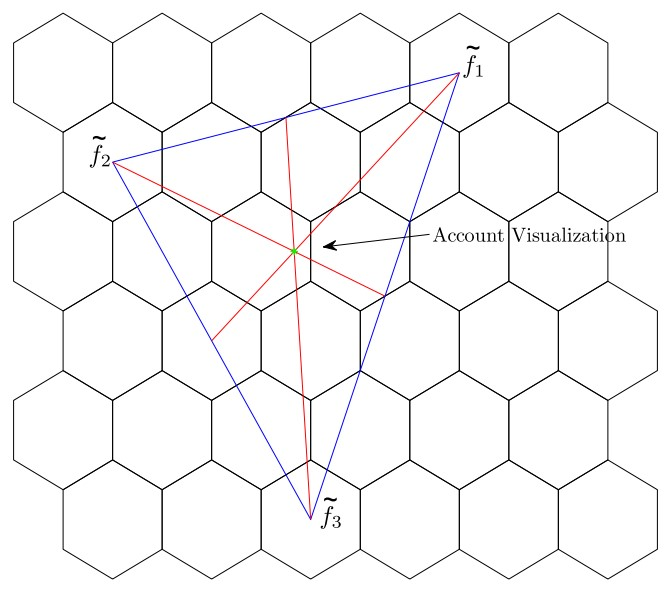
\includegraphics[width=1\textwidth]{images/SOM_user_acc_visualisation.jpg}
        \subcaption{User account representation}   
        \label{fig:SOM_user_acc_visualisation}
    \end{subfigure}
    \begin{subfigure}[t]{0.5\textwidth}
        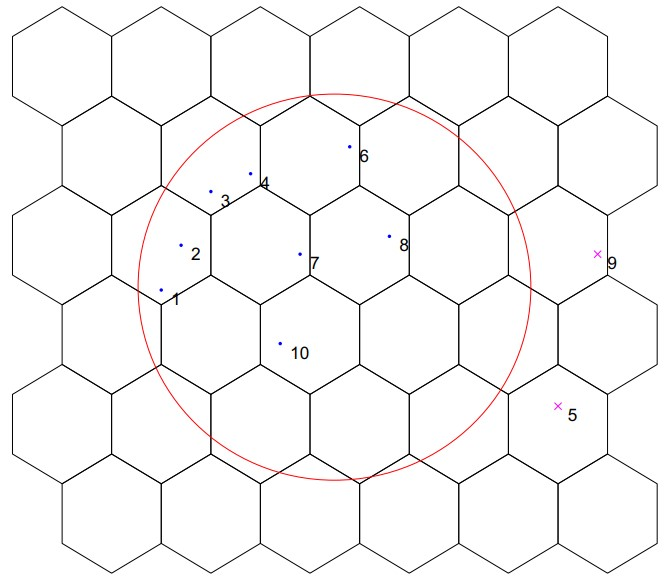
\includegraphics[width=1\textwidth]{images/SOM_threshold_bin_classification.jpg}
        \subcaption{Threshold-classification of instances}
        \label{fig:SOM_threshold_bin_classification}
    \end{subfigure}
    \caption{\ac{SOM} visualisation from \cite{fd_SOM}}
\end{figure}

The $i$th user account is represented by the centroid $c_i$ on the \ac{SOM} grid, which is calculated in \eqref{eq:acc_representation} and visualised in \autoref{fig:SOM_user_acc_visualisation}.
There can be accounts that do not correspond to a particular neuron (i.e. hexagon) in a \ac{SOM} grid. 
It is also possible that multiple similar accounts share a neuron.
%
\begin{ceqn}
    \begin{equation}
    \label{eq:acc_representation}
        c_i = \frac{1}{m}\sum^{m}_{j=1} \tilde f_{i,j}
    \end{equation}
\end{ceqn}
%
According to \cite{fd_SOM}, the reduction of the inner-dimensionality of features from \eqref{eq:feature_projection} does not reduce the amount of information, since the majority of records of a fraudulent user account are fraudulent themselves.

Each entry of the U-matrix of a \ac{SOM} corresponds to a neuron in the \ac{SOM} grid. Its value is the average dissimilarity between the neuron and its neighbours.
Hence, a so-called ridge (sequence of high values) in the U-matrix represents a borderline separating the data clusters in the corresponding \ac{SOM} grid.
\autoref{fig:U_Matrix} is a visualisation of an U-matrix. The colour of a hexagon corresponds to the value of the neuron in the U-matrix (cf. legend on the right side). 
Red coloured hexagons correspond to the highest values of average dissimilarity of neurons in the U-matrix. Hence, the group of red hexagons is a ridge. 
Although the closest user accounts below the ridge are considered non-fraudulent, the user accounts with more distance to the ridge (and below it) are marked as fraudulent. 
Thus, the ridge in fact separates the two clusters.

\begin{figure}[http]
    \begin{center}
      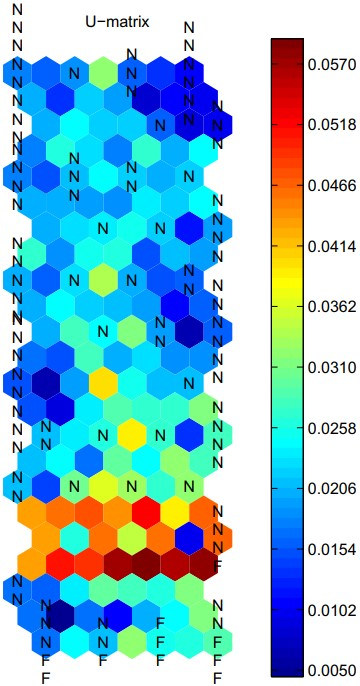
\includegraphics[scale=0.3]{images/SOM_U_Matrix_vis.jpg}
      \caption{Visualisation of U-matrix from \cite{fd_SOM}. The letter \textit{N} marks non-fraudulent user accounts, whereas \textit{F} marks fraudulent user accounts. The coloured hexagons correspond to the values of the average dissimilarity of neurons and their neighbours in the U-matrix.}
      \label{fig:U_Matrix}
    \end{center}
\end{figure}

As stated in \cite{fd_SOM}, the classification of (non-)fraudulent instances is performed by a threshold-type binary classification technique. 
Visually, the threshold of the circle illustrated in \autoref{fig:SOM_threshold_bin_classification} with centre $c$, which is the centroid of the entire \ac{SOM} grid and radius $\tau$, which is calculated in \eqref{eq:radius_threshold}.
$v_{max}$ is the \ac{SOM} neuron corresponding to the maximal value in the U-matrix of the \ac{SOM} and $d(.,.)$ is a chosen dissimilarity measure.
All points outside the circle are considered fraudulent user accounts and respectively all points within the threshold are considered normal user accounts.
%
\begin{ceqn}
    \begin{equation}
    \label{eq:radius_threshold}
        \tau = d(c, v_{max})
    \end{equation}
\end{ceqn}
%
\begin{ceqn}
    \begin{equation}
    \label{eq:identify_anomalies}
        \varphi(a_i) = 
        \begin{cases}
          \text{true} & \text{for } d(c_i, c) > \tau\\
          \text{false} & \text{for } d(c_i, c) \le \tau\\
        \end{cases}   
    \end{equation}
\end{ceqn}
%
\eqref{eq:identify_anomalies} classifies a user account $a_i$ as either fraudulent (return value true) or non-fraudulent (return value false).